\documentclass[a4paper,12pt,oneside,bibtotoc,numbers=noenddot]{scrreprt}

%Pakete
\usepackage[latin9]{inputenc}
\usepackage[ngerman]{babel}
\usepackage{listings}
\usepackage{graphicx}
\usepackage{BachelorThesis}

% Allgemeine Informationen
\newcommand\mytitle{Titel der Arbeit}
\newcommand\myauthor{Name des Autors oder der Autoren}
\newcommand\mydepartment{Informatik und Elektrotechnik}
\newcommand\myinstitute{Hochschule Zittau/G\"{o}rlitz}
\newcommand\mytutor{Name und Titel des betreuenden Professors}
\newcommand\mySecondTutor{Name und Titel des betrieblichen Betreuers}

% Abstracts
\newcommand\mysubject{Das deutsche Abstract.}
\newcommand\mysubjectenglish{The english abstract.}

% PDF-Einstellungen
\hypersetup
{
	pdftitle = \mytitle,
	pdfsubject = \mysubject,
	pdfauthor = \myauthor,
	pdfkeywords = {},
	colorlinks = {true},
	pdfborder = 0 0 0
}

\begin{document}
\nocite{*}

%
\pagenumbering{alph}
\begin{titlepage}
\thispagestyle{empty} 
 \begin{center}
 \vspace{2.0cm} 
 {\bfseries \huge Ausf�hrungsplanoptimierung in PostgreSQL\\}
 \vspace{3.0cm} 
 {\bfseries \huge Belegarbeit\\}
 \vspace{3.0cm}
 {\normalsize eingereicht am Fachbereich\\}
 {\bfseries \Large Informatik\\}
 {\normalsize der Hochschule Zittau/G�rlitz (HAW)\\}
 \vspace{1cm}
 {\normalsize als Pr�fungsleistung im Fach\\}
 {\bfseries \Large Fortgeschrittene Datenbank-Konzepte 2\\}
 \vspace{1cm}
 {\normalsize vorgelegt von:\\}
 {\bfseries \Large Christof Ochmann (35989)\\
 Ingo K�rner (40586)\\}
 \vspace{1cm}
 {\normalsize  G�rlitz, 9. Juli 2012\\}
 \vspace{0.5cm}
 Betreuer:	Prof. ten Hagen\\
 \vfill
\end{center}
\end{titlepage}

%
%% Kurzreferat
\thispagestyle{empty}
\section*{Abstract}\label{Abstract}
Diese Arbeit baut auf das Projekt Datenbankkonfigurationen\footnote{https://dl.dropbox.com/u/608146/ADBC1\%20OLAP.pdf}, dass w�hrend der Vorlesungsreihe ADBC1 erstellt wurde, auf.
Im Projekt Datenbankkonfigurationen wird untersucht, wie sich die Ausf�hrungsgeschwindigkeit von Abfragen steigern l�sst.
Im Projekt Ausf�hrungsplanoptimierung in PostgreSQL wird dar�berhinaus untersucht, welche Ausf�hrungspl�ne f�r bestimmte Konfigurationen und bestimmte Queries erzeugt werden. Und wie sich diese Pl�ne auf die Ausf�hrungs\-geschwin\-digkeit von SQL-Queries auswirken.
In beiden Projekten wird nur der Bereich OLAP f�r Kaltstarts von Abfragen betrachtet.
Diese Arbeit behandelt nur Datenbankkonfigurationen, die Einfluss auf den Ausf�hrungsplan haben. F�r alle Konfigurationen die keinen Einfluss haben, wird der Standardwert von PostgreSQL beibehalten.
Ziel der Arbeit ist, Annahmen �ber Ausf�hrungspl�ne zu treffen, diese theoretisch zu begr�nden und dann auch praktisch zu untersuchen. Anhand der praktischen Untersuchungen werden die aufgestellten Hypothesen best�tigt oder wiederlegt.
F�r wiederlegte Hypothesen wird eine Begr�ndung gesucht.

%\mysubject
%\section*{Abstract}
%\mysubjectenglish

\pagenumbering{Roman}
\tableofcontents
\listoffigures
\lstlistoflistings

\begin{listofacronyms}
\acronym{DBMS}{Datenbankmanagementsystem}
\acronym{ERD}{Entity-Relationship Diagram}
\acronym{OLAP}{Online Analytical Processing}
\acronym{SQL}{Structured Query Language}

\end{listofacronyms}

\begin{flushleft}
\begin{thebibliography}{sotief}
\bibitem{bib1}{Martin, Robert C. (2008): Clean Code: A Handbook of Agile Software Craftsmanship. Prentice Hall International}

\bibitem{bib2}{Freeman, Eric (2007): Entwurfsmuster von Kopf bis Fu�. O'REILLY}

\bibitem{bib4}{\begin{verbatim}http://www.postgresql.org/ (08.06.2012)\end{verbatim}} 

\bibitem{bib5}{\begin{verbatim}http://wiki.postgresql.org/ (08.06.2012)\end{verbatim}} 



\end{thebibliography}
\end{flushleft}

\newpage
\pagestyle{chapterStyle}
\pagenumbering{arabic}

\chapter{Theorie}
\section{Einleitung}\label{Einleitung}

\section{Aufgabenstellung}\label{Aufgabenstellung}
In diesem Projekt werden Ausf�hrungspl�ne f�r bestimmte Queries untersucht. Dazu werden Queries ausgew�hlt, die im Bereich OLAP und Data Warehouse angesiedelt sind. Als Grundlage wird ein Datenbankentwurf f�r ein Projekt aus der Vorlesungsreihe XML genommen.
Die Tabellen sollen mit Testdaten gef�llt werden. Dazu ist der Datengenerator aus dem Projekt Datenbankkonfigurationen anzupassen.
Die Abfragen werden auf den gef�llten Tabellen angewendet. Die Ausf�hrungspl�ne, die daf�r erzeugt werden, werden nach Performancegesichtspunkten untersucht.
\section{Relevanz des Forschungsgegenstandes}\label{RelevanzDesForschungsgegenstandes}
Der Forschungsgegenstand dieser Arbeit ist, Annahmen �ber erzeugte Ausf�hr\-ungs\-pl�ne von Abfragen zu treffen und gegebenfalls wiederlegte Annahmen zu erkl�ren.
Der Forschungsgegenstand ist relevant, da bisher keine konkreten Aus\-f�hr\-ungs\-pl�ne f�r die gew�hlten Abfragen vorliegen. Ziel dieser Foschung ist es, Ausf�hrungspl�ne zu finden, die die h�chste Ausf�hrungsgeschwindigkeit f�r alle Abfragen bringt. 

Um die optimalen Ausf�hrungspl�ne zu finden, muss sich vertiefend in eine PostgreSQL
eingearbeitet werden. Das geschieht z.B. unter Zuhilfenahme von B�chern und
Online-Ressourcen. In diesen Medien ist der Forschungsstand zur Erstellung von
Ausf�hrungspl�nen dokumentiert. Bei der Anpassung des Datengenerators m�ssen
dar�berhinaus technische Probleme gel�st werden.
\section{Der aktuelle Wissensstand}\label{DerAktuelleWissensstand}
\cite{bib4}
\section{PostgreSQL}\label{PostgreSQL}
Da im Projekt Datenbankkonfigurationen bereits viel Erfahrung mit MySQL gesammelt wurde, wird im aktuellen Projekt nun nach einem DBMS gesucht, mit qualitativ �hnlichen Eigenschaften zu MySQL. Ziel ist dabei auch andere DBMS kennen zu lernen. F�r die Untersuchung der Ausf�hrungspl�ne wird dazu PostgreSQL gew�hlt, ein freies, objektrelationales Datenbankmanagementsystem f�r das mit PgAdmin auch eine grafische Benutzeroberfl�che zur Verf�gung steht.
\section{Was ist ein Ausf�hrungsplan?}\label{WasIstEinAusfuehrungsplan}
In einem Ausf�hrungsplan wird beschrieben, in welchen Schritten ein DBMS einen Query ausf�hrt. Auch die Reihenfolge der Schritte wird dabei angegeben.
Da in einem Query nur beschrieben steht, was im Ergebnis gew�nscht ist, aber kein Algorithmus, wie dieses Ergebnis errechnet werden soll, gibt es viele verschiedene M�glichkeiten, zu dem Ergebnis zu kommen. Das DBMS soll dabei den Ausf�hrungsplan finden, der das Ergebnis effizient errechnet.

Technisch betrachtet, ist der Ausf�hrungsplan ein Baum. Die Abarbeitung des Ausf�hrungsplans beginnt bei seinen Bl�ttern. In den Bl�ttern des Baumes stehen die Zugriffspfade (access paths).
Der Zugriffspfad wird durch den Scan-Algorithmus angegeben. Ein Scan-Algorithmus gibt an, wie eine Tabelle durchlaufen wird.
%\section{Die Abarbeitung von Abfragen in PostgreSQL}
\begin{enumerate} 
\item \textbf{Empfang des SQL-Befehls} \\
Nachdem der SQL-Befehl �ber eine Netzwerkverbindung �bertragen wurde, findet die Kodierungsumwandlung statt, 
und die weiteren Phasen der Abarbeitung sehen den Befehl in der Serverkodierung. Hierbei gibt es nur sehr
geringe Optimierungsm�glichkeiten. Es k�nnen theoretisch CPU-Zyklen gespart werden, wenn die Clientkodierung 
gleich der Serverkodierung ist, ansonsten wird eine Konvertierung durchgef�hrt. Diese Auswirkungen sind jedoch sehr gering.
Der Parameter \textit{client\_encoding} informiert den Server dar�ber, welche Kodierung die ankommenden Befehle haben 
und welche Kodierung das Anfrageergebnis haben soll, welches an den Client gesendet wird. Die Voreinstellung 
gibt an welche Kodierung der Server intern verwendet.

\item \textbf{Parser} \\
In dieser Abarbeitungsphase wird die kodierte Befehlszeichenkette durch einen internen Parse-Baum dargestellt. 
Des Weiteren wird die Befehlszeichenkette auf semantische Bedingungen �berpr�ft und etwas bearbeitet. Die SQL-Befehle werden dann 
aufgeteilt in sogenannte optimierbare Anweisungen(SELECT, INSERT, UPDATE und DELETE) und Hilfsanweisungen.
Die Hilfsanweisungen werden sp�ter direkt ausgef�hrt und sie erzeugen keine Ausgabe. Dagegen kommen die optimierbaren 
Anweisungen in den Rewriter. F�r den Parser gibt es von der Anwenderseite keine M�glichkeit die Geschwindigkeit 
zu optimieren. 


\item \textbf{Query Rewriter} \\
Der Rewriter wendet die Anfrageumschreibregeln(Query Rewrite Rules) an. Dabei werden die Sichten(Views) und andere
benutzerdefinierte Regeln aufgel�st, in die Anfrage eingebaut und im Parse-Baum ersetzt. Da der Rewriter 
vor dem Planer angesiedelt ist, bekommt der Planer es nicht mit, ob die Anfrage aus einer Sicht kam oder nicht. Mit der 
Erstellung einer Sicht hat man somit keinen Optimierungsvorteil.

\item \textbf{Planer / Optimizer} \\
Der Planer bekommt den m�glicherweise umgeschriebenen Parse-Baum und hat die Aufgabe einen Ausf�hrungsplan(execution plan) zu erstellen, der ebenfalls ein Baum ist.
Der Ausf�hrungsplan beschreibt wie auf die Tabellen zugegriffen werden soll, also welche Indexe und Join-Algorithmen verwendet werden sollen und in welcher Reihenfolge. Es soll m�glichst der optimalste und schnellste Ausf�hrungsplan gefunden werden. 

\item \textbf{Executor} \\ 
Der vom Planer auserw�hlte Ausf�hrungsplan wird vom Executor ausgef�hrt. Dabei werden Zugriffsrechte auf Tabellen und andere Objekte sowie Constraints gepr�ft. Die Laufzeit der Ausf�hrung h�ngt nicht nur davon ab ob der Plan gut ist, sondern auch von der gesamten Systemkonfiguration.

\end{enumerate}
%\section{Ausf�hrungsplan ver�ndern}
In PostgreSQL hat der Anwender keine M�glichkeit selbst einen Plan vorzugeben, aber
mit bestimmten Parametern kann man den Anfrageplaner beeinflussen und somit den Ausf�hrungsplan ver�ndern. Man kann einzelne Plantypen ausschalten und den Planer dazu bringen nur die aktivierten Plantypen zu verwenden. Die Parameter werden w�hrend einer Datenbanksitzung mit dem SET-Befehl gesetzt: 
\\
z.B. \textbf{SET enable\_seqscan TO off} \\


In der Voreinstellung sind alle Plantypen an und k�nnen vom Planer benutzt werden. Die folgende Auflistung zeigt die verschiedenen Plantypen und ihre Bedeutung: \\
\begin{itemize}
\item enable\_seqscan: \\
Wenn der Planer zu sequenziellen Pl�nen tendiert, kann man mit diesem Parameter die Verwendung von indexbasierten Pl�nen erzwingen. Die sequenziellen Pl�ne werden zwar nicht ganz abgeschaltet, aber sie werden extrem hoch bewertet und erscheinen zu aufwendig f�r den Planer um sie zu nutzen. Auf die selbe Art und Weise k�nnen die folgenden Parameter den Planer beeinflussen: 

\item enable\_indexscan: \\
Hiermit werden die indexbasierten Pl�ne aktiviert bzw. deaktiviert.

\item enable\_bitmapscan: \\
Auch das Aktivieren und Deaktivieren von Bitmap Index Scans ist m�glich.

\item enable\_nestloop:\\
Aktivierung bzw. Deaktivierung von Nested-Loop-Joins. 

\item enable\_hashjoin: \\
Aktivierung bzw. Deaktivierung von Hash-Join-Plantypen.

\item enable\_mergejoin: \\
Aktivierung bzw. Deaktivierung von Merge-Join-Plantypen.

\item enable\_hashagg: \\
Aktivierung bzw. Deaktivierung von Hash-basierter Aggregierung.

\item enable\_sort: \\
Sortieroperationen werden vom Planer nicht ber�cksichtigt wenn dieser Parameter deaktiviert ist. Es kann aber vorkommen, dass sie trotzdem im Anfrageplan vorkommen wenn keine Alternativen herangezogen werden k�nnen.

\item enable\_tidscan: \\
Aktivierung bzw. Deaktivierung von TID-basierten Plantypen.
\end{itemize}
%\section{Kostenparameter}

Au�er den Plantypen gibt es noch die Kostenparameter, die den erwarteten I/O und CPU-Aufwand z�hlen. �ndert man diese Konfigurationsparameter, dann werden die Anfragen andere Plankosten haben und es wird eventuell ein anderer, g�nstigerer Ausf�hrungsplan gew�hlt. Man muss die Kostenfaktoren so einstellen, dass der Plan dem Planer auch am schnellsten erscheint und somit ausgew�hlt wird.

Die Voreinstellungen dieser Parameter stellen das ungef�hre Verhalten eines typischen Computers dar und m�ssen lediglich an das eigene System angepasst werden. Jedoch gibt es kein Benchmark-Programm, mit dem man diese Einstellungen automatisch vornehmen k�nnte. 
In der Regel sind keine weitreichenden �nderungen an diesen Parametern notwendig, es sein denn man nutzt diese als Mittel um einen anderen Ausf�hrungsplan zu erzwingen. Die �nderungen sollten in kleinen Schritten und mit ausf�hrlichen Tests f�r alle in Frage kommenden Anfragen vorgenommen werden, denn eine falsche Konfiguration kann bei bestimmten Anfragen zu einem hohen Ressourcenverbrauch f�hren. Die wichtigsten Kostenparameter sind:

\begin{itemize}

\item \textbf{seq\_page\_cost}: \\
Wird eine Page von der Platte gelesen, entsteht Aufwand, der mit diesem Parameter definiert ist. Er gibt die Kosten f�r das sequenziellen Lesen einer Page(typischerweise 8kb) w�hrend einer laufenden Leseanweisung an, die Voreinstellung f�r diesen Parameter ist 1.0.

\item \textbf{random\_page\_cost}: \\
Der Parameter gibt an, um wie viel aufw�ndiger es ist, Pages in zuf�lliger Reihenfolge zu lesen, wie es bei Indexscans vorkommt (gemessen am sequentiellem Lesen von Pages). Die Voreinstellung  ist 4.
Die Parameter seq\_page\_cost und random\_page\_cost kann man sich vereinfacht als Kosten f�r sequenzielle Scans und Indexscans vorstellen. Indexscans sind langsamer als das sequenzielle Lesen, daf�r aber muss man in der Regel bei den Indexscans nicht so viele Seiten lesen. Mit diesen Parametern entscheidet der Planer zwischen Index und nicht Index.
Die Voreinstellung besagt, dass ein Indexscan viermal langsamer ist als der sequenzielle Scan. Dieser Wert kann jedoch bei schnellen Festplatten zu hoch sein und es wird empfohlen den Wert pauschal auf 2.0 oder 3.0 herunterzusetzen.
Wenn sich die Datenbank komplett im Hauptspeicher befindet, ist es sinnvoll die beiden Parameter gleichzusetzen, da der Aufwand in diesem Fall gleich ist.

\item \textbf{cpu\_tuple\_cost}: \\
Hiermit werden die Kosten f�r das Verarbeiten einer Tabellenzeile durch die CPU definiert. Die Voreinstellung ist 0.01 und dieser Wert wird in der Regel sehr selten ver�ndert.

\item \textbf{cpu\_index\_tuple\_cost}: \\ 
Dieser Parameter definiert die Kosten f�r das Verarbeiten eines Indexeintrags durch die CPU w�hrend eines Indexscans. Auch dieser Parameter wird sehr selten ver�ndert und ist auf 0.005 voreingestellt.

\item \textbf{cpu\_operator\_cost}: \\
Dieser Konfigurationsparameter gibt die Kosten f�r das Ausf�hren eines Operators oder einer Funktion an. Die Voreinstellung ist 0.0025 und wird in der Regel sehr selten ver�ndert.

\item \textbf{effective\_cache\_size}: \\ 
Dieser Parameter gibt an, wie viel Cache-Speicher f�r eine Anfrage vom Betriebssystem bereitgestellt werden. Es ist nur eine Vermutung und es wird kein Speicher angelegt. Der Planer sieht anhand dieses Parameters ob ein Index im Hauptspeicher h�chstwahrscheinlich gecached ist, oder noch von der Festplatte gelesen werden muss. Daraufhin entscheidet der Planer ob ein indexbasierter Zugriffspfad zu w�hlen ist oder ob nicht eine andere Alternative kosteng�nstiger ist. Ein hoher Wert sorgt also daf�r, dass mehr Indexscans verwendet werden. Die Voreinstellung betr�gt 128 MByte.

\end{itemize}
%\section{Indexe}

Ein Index auf eine Spalte lohnt sich nur bei hoher Selektivit�t. Wenn die Selektivit�t nicht hoch ist, muss sowieso die gesamte Tabelle durchgegangen werden, d.h. jeder Block angefasst werden.
Wenn der Planer mit analyze genug Statistiken hat, entscheidet er, ob er den Index verwendet oder nicht.

Ein Index lohnt sich nicht, wenn man viele Ergebnisse erwartet und einen nur die ersten zehn Zeilen interessieren. Denn dann kann sich der Planer das durchhashen und sortieren ersparen.
Der Planer sollte den Index nicht verwenden, wenn ein Limit von z.B. zehn angegeben wurde.

\subsection{Indextypen}

Von PostgreSQL werden derzeit vier Indextypen unterst�tzt:

\begin{itemize}

\item B-tree: \\
Es ist die Implementierung des B+-Baums und der Standardindextyp. Er kann alle Anfragen mit den Vergleichsoperatoren( <, <=, =, >=, >) und den Konstrukten wie BETWEEN und IN bearbeiten.

\item Hash: \\ 
Dieser Indextyp verwendet eine Hashtabelle und bedient nur Anfragen mit dem Gleichheitsoperator(=). Er bietet keine bessere Geschwindigkeit als B-tree und wird heutzutage haupts�chlich nur bei Experimenten verwendet. 

\item GiST: \\
Bei GiST handelt es sich um eine universelle Schnittstelle, um verschiedene anwendungsspezifische Indextypen selbst definieren zu k�nnen. Zwei Anwendungen davon sind PostGIS und OpenFTS(Open Source Full Textj Search). Man verwendet diesen Indextyp um beispielsweise Geodaten zu sortieren oder bei der Volltextsuche.

\item GIN: \\
Hierbei handelt es sich um einen invertierten Index, der Werte mit mehreren Schl�sseln wie beispielsweise Arrays und Listen indizieren kann.

\end{itemize}

\subsection{Pl�ne mit Bitmap Index Scan}

Der reine Indexscan eignet sich am besten dort, wo die Selektivit�t sehr hoch ist und der reine Sequential Scan sollte bei niedriger Selektivit�t verwendet werde, also dann wenn die Tabelle komplett oder fast komplett gelesen werden soll. Der Bitmap Index Scan dagegen soll das gesamte Spektrum zwischen Index- und Sequential Scan abdecken, also die Vorteile von beiden Indextypen kombinieren. 

\begin{verbatim}
EXPLAIN Select *
from public.user u
where u.gender = 'w'
AND u.birthday between '01.01.1986' AND '31.12.2013'
\end{verbatim}

Query Plan:
\begin{verbatim}
"Bitmap Heap Scan on "user" u  (cost=64.62..236.66 rows=1412 width=61)"
"  Recheck Cond: ((birthday >= '1986-01-01'::date) 
		AND (birthday <= '2013-12-31'::date))"
"  Filter: (gender = 'w'::text)"
"  ->  Bitmap Index Scan on user_birthday  
				(cost=0.00..64.27 rows=2802 width=0)"
"        Index Cond: ((birthday >= '1986-01-01'::date) 
					AND (birthday <= '2013-12-31'::date))"
\end{verbatim}
Wie man bei diesem Ausf�hrungsplan sehen kann, besteht der Bitmap Index Scan aus zwei Schritten. Zuerst werden alle Treffer aus dem Index ermittelt und in einer Bitmap im RAM zwischengespeichert und sortiert. Anschlie�end werden die Treffer beim Bitmap Heap Scan in der Tabelle der Reihe nach aufgesucht. Die Spr�nge zwischen Tabelle und Index werden somit verhindert. Der Bitmap Index Scan liefert dem Bitmap Heap Scan die Eingabe und ist ihm somit untergeordnet, was man bei einem Ausf�hrungsplan an dem Pfeil erkennen kann. Die Startkosten f�r den Bitmap Heap Scan sind gr��er null, d.h., dass der Bitmap Index Scan abgeschlossen sein muss, bevor der Bitmap Heap Scan seine Arbeit beginnen kann.

%\section{Plananalyse}

Mit dem Befehl EXPLAIN gefolgt von der eigentlichen Anfrage k�nnen die Ausf�hrungpl�ne angesehen werden:

Beispiel1 ohne Indexe:
\begin{verbatim}
EXPLAIN Select u.userId, u.name, u.email, u.gender, u.birthday
from public.user u, public.event e, public.participation p
where e.eventname = 'event1'
AND e.eventid = p.eventid
AND p.userid = u.userid;
\end{verbatim}

\begin{verbatim}
"Hash Join  (cost=480.53..506.29 rows=1 width=38)"
"  Hash Cond: (u.userid = p.userid)"
"  ->  Seq Scan on "user" u  (cost=0.00..22.00 rows=1000 width=38)"
"  ->  Hash  (cost=480.52..480.52 rows=1 width=8)"
"        ->  Hash Join  (cost=279.01..480.52 rows=1 width=8)"
"              Hash Cond: (p.eventid = e.eventid)"
"              ->  Seq Scan on participation p  
									(cost=0.00..164.00 rows=10000 width=16)"
"              ->  Hash  (cost=279.00..279.00 rows=1 width=8)"
"                    ->  Seq Scan on event e  
													(cost=0.00..279.00 rows=1 width=8)"
"                          Filter: (eventname = 'event1'::text)"

\end{verbatim}

\begin{itemize}
\item Die erste Zahl nach dem "`cost"' sind die Startkosten. Es ist der gesch�tzte Aufwand, den der Executor investieren muss, bevor der Planknoten Ergebnisse produzieren kann. Eine 0.00 bedeutet, dass bei einem sequenziellen Scan die Ergebnisse sofort ausgegeben werden, sobald der Scan ausgef�hrt wird.  

\item Die zweite Zahl ist der gesch�tzte Aufwand f�r die Abarbeitung des Planknotens und somit die interessante von den beiden Zahlen.

\item Die Zeilenzahl(rows) ist eine Sch�tzung �ber die Anzahl der ausgegebenen Ergebniszeilen. Anhand dieser Zahl wird die Abw�gung getroffen, ob ein Indexscan g�nstiger ist oder auch nicht und ob andere Planvarianten infrage kommen. 

\item Die letzte Zahl gibt die Gr��e der Ergebniszeile in Bytes an(width). Man kann mit Hilfe der Zeilenzahl(rows) den Speicherbedarf der Ergebnismenge vorhersehen(rows * width).
\end{itemize}

Die gesch�tzten Kosten f�r einen sequenziellen Scan der Tabelle "`user"', die in unserem Beispiel1 auf 22.00 gesch�tzt werden,  lassen sich mit Hilfe folgender Anfrage in PostgreSQL leicht berechnen: \\ 

SELECT relpages, reltuples FROM pg\_class WHERE relname = 'user'
\\

Das Ergebnis dieser Anfrage ist: \\
relpages: 12 \\
reltuples: 1000

Das bedeutet, dass die Tabelle "`user"' aus 12 Diskpages besteht und 1000 Zeilen enth�lt.

Der gesch�tzte Aufwand f�r die Abarbeitung des Planknotens, der nur aus einem sequenziellen Scan besteht (Seq Scan on "`user"' u  (cost=0.00..22.00 rows=1000 width=38)
), wird wie folgt berechnet:

(Anzahl der Diskpages(je 8 KByte) x seq\_page\_cost) + ( rows x cpu\_tuple\_cost)) 
In unserem Beispiel1:
(12 * 1.0) + (1000 * 0.01) = 22 

Also die Anzahl der Seiten mal die Kosten f�r das sequenzielle Lesen einer Page plus die Anzahl der Zeilen mal die Kosten f�r die Abarbeitung einer Zeile in der CPU.
%\section{Planvergleich}

Mit dem Befehl \textbf{EXPLAIN ANALYZE} kann man die gesch�tzten Kosten mit den Ergebnissen der Ausf�hrung vergleichen. Die Anfrage wird auch auch tats�chlich ausgef�hrt:

\begin{verbatim}
"Hash Join  (cost=480.53..506.29 rows=1 width=38) 
		(actual time=19.767..20.204 rows=1 loops=1)"
"  Hash Cond: (u.userid = p.userid)"
"  ->  Seq Scan on "user" u  
		(cost=0.00..22.00 rows=1000 width=38) 
		(actual time=0.029..0.279 rows=1000 loops=1)"
"  ->  Hash  (cost=480.52..480.52 rows=1 width=8) 
				(actual time=19.439..19.439 rows=1 loops=1)"
"        Buckets: 1024  Batches: 1  Memory Usage: 1kB"
"        ->  Hash Join  (cost=279.01..480.52 rows=1 width=8) 
							(actual time=9.220..19.428 rows=1 loops=1)"
"              Hash Cond: (p.eventid = e.eventid)"
"              ->  Seq Scan on participation p  
									(cost=0.00..164.00 rows=10000 width=16) 
									(actual time=0.037..4.178 rows=10000 loops=1)"
"              ->  Hash  (cost=279.00..279.00 rows=1 width=8) 
									(actual time=9.109..9.109 rows=1 loops=1)"
"                    Buckets: 1024  Batches: 1  Memory Usage: 1kB"
"                    ->  Seq Scan on event e  
										(cost=0.00..279.00 rows=1 width=8) 
										(actual time=0.040..9.102 rows=1 loops=1)"
"                          Filter: (eventname = 'event1'::text)"
"Total runtime: 20.386 ms"

\end{verbatim}

Die Zahlen in der ersten Klammer sind dieselben wie bei \textbf{EXPLAIN} und die Daten in der zweiten Klammer enthalten analog zu den Kosten die tats�chliche Ausf�hrungszeit sowie die tats�chliche Anzahl der Zeilen. Der Parameter loops zeigt an wie oft dieser Teilplan ausgef�hrt wird, spielt jedoch erst bei Joins eine Rolle, denn bei einfachen Anfragen ist die Zahl logischerweise eine 1. 

Bei \textbf{EXPLAIN ANALYZE} ist es am wichtigsten darauf zu achten, ob die Zeilensch�tzung richtig war. Bei gr��eren Abweichungen m�ssen die Statistiken verbessert werden.
%\section{Statistiken}

Der Planer sammelt Statistiken um die Anzahl der zu erwartenden Ergebniszeilen zu ermitteln. Relevant dabei ist die Anzahl der Zeilen in der Tabelle, sowie die Anzahl der von der Tabelle belegten Bl�cke. Diese Daten stehen in der Systemtabelle pg\_class und der Planer kann mit Hilfe dieser Informationen die Anzahl der Zeilen f�r einen sequenziellen Scan �ber eine Tabelle, sowie den Speicher- und I/O-Aufwand ermitteln. Aktuell gehalten werden die Statistiken von den Befehlen \textbf{VACUUM} und \textbf{ANALYZE}, sowie von \textbf{CREATE INDEX}.
Meistens jedoch werden die Tabellen nicht komplett gelesen, sondern m�ssen nach bestimmten Kriterien z.B. mit der WHERE-Klausel ausgew�hlt werden. Dazu muss der Planer weitere Statistiken sammeln, die in der Tabelle pg\_statistics stehen und mit der folgenden Anfrage eingesehen werden k�nnen: 
\begin{verbatim}
SELECT * FROM pg\_stats WHERE tablename = 'user' 
					AND attname = 'birthday'
\end{verbatim}

Das Ergebnis dieser Anfragen sind N�herungswerte und beziehen sich immer nur auf eine Spalte. Die interessantesten sind: 

\begin{itemize}

\item  \textbf{n\_distinct} = 80: Die Zahl bedeutet, dass die Tabelle 80 unterschiedliche Werte enth�lt. 
\item  \textbf{most\_common\_vals} = 1951-02-01, 1947-02-01, usw.: Ein Array mit den h�ufigsten Werten in der Tabelle.
\item \textbf{correlation} = 0.016471: Eine Korrelation zwischen der logischen Reihenfolge der Werte und der Reihenfolge auf der Festplatte. Ein Wert der nah bei -1 oder +1 liegt bedeutet, dass Indexscans g�nstiger sind, weil die Festplattenzugriffe nicht so weit auseinander liegen.

\end{itemize}
\section{Die drei Scan-Algorithmen}\label{DieDreiScanAlgorithmen}
Ein Scan-Algorithmus arbeitet immer nur auf einer einzelnen Tabelle. In Postgre\-SQL gibt es die folgenden drei Scan-Algorithmen:

\begin{enumerate}
\item sequential scan (full table scan) \\
Der Inhalt der Tabelle wird komplett gelesen. Er wird blockweise vom Sekund�rspeicher wie z.B. einer Festplatte in den Arbeitsspeicher geholt.

\item index scan \\
Hat eine Tabelle einen Index, kann er verwendet werden, um die Tupel sortiert zu lesen. Bei einem Index Scan werden Bl�cke auch mehrmals gelesen, wenn der Inhalt der Tabelle nicht auch sortiert in den Bl�cken vorliegt. Das ist relativ teuer und nur f�r kleine Treffermengen geeignet. Ein Index-Scan eignet sich bei einer hohen Selektivit�t eines Selects.

\item bitmap index scan \\
Hier wird der Index gescannt und ein Bitmap mit den getroffenen Blocknummern erzeugt. Das Bitmap der Blocknummern wird dann aufsteigend sortiert. Die Tabelle wird anhand der sortierten Bitmap-Blocknummern aufsteigend gescannt. Das ist nur m�glich, wenn Indexe f�r die betreffenden Spalten existieren.
\end{enumerate}
\section{Die drei Join-Algorithmen}\label{DieDreiJoinAlgorithmen}
In den Knoten des Ausf�hrungsplanes stehen Datenbankoperatoren wie Projek\-tion, Selektion, Kreuzprodukt, Vereinigung, Differenz oder Umbenennung.

Die Hintereinanderausf�hrung der Operationen kartesisches Produkt und Selektion wird Join genannt. Joins werden im DBMS intern �ber Join-Algorithmen realisiert. Join-Algorithmen verkn�pfen Tabellen paarweise miteinander.

In PostgreSQL gibt es drei grundlegende JOIN-Algorithmen:

\begin{enumerate}
\item nested loop join \\
F�r jede Zeile aus der treibenden Tabelle wird die innere Tabelle einmal durchlaufen. Wenn die innere Tabelle indiziert ist, kann sie mit einem Index-Scan durchlaufen werden.
Ein Nested Loop Join kann sehr kostenintensiv werden, wenn er die innere Tabelle mehrmals lesen muss.
Wenn auf der inneren Tabelle ein Index-Scan erfolgen kann, oder die innere Tabelle sehr klein ist, kann sich diese durch vorherige Anfragen im Cache befinden und so schnell abgearbeitet werden.
Wenn es sich um einen sequentiellen Scan handelt, der alle Zeilen vergleicht, dann muss die innere Tabelle u.U. so oft von der Festplatte gelesen werden, wie die treibende Tabelle Zeilen hat.
Wird nur die erste �bereinstimmende Zeile gesucht, ist der Nested Loop Join schneller als andere Joins, die vorher erst ihr komplettes Ergebnis berechnen m�ssen, bevor sie den ersten Treffer zur�ckgeben k�nnen.
Der Nested Loop Join verlangt vor dem Query keinerlei Investition, wie Hashing oder Sortierung.

\item hash join \\
F�r einen Hashjoin m�ssen beide Tabellen als Hash-Tabelle vorliegen. Das setzt vorraus, dass bevor ein Hash Join eingesetzt werden kann, die Tabellen durchgehasht wurden, d.h. ein Hashwert f�r das sp�tere Join-Attribut gebildet wird. Wie der Nested Loop Join ist der Hash-Join besonders performant, wenn der Gr��enunterschied zwischen treibender Tabelle und innerer Tabelle gro� ist und die kleinere Tabelle komplett in den Speicher passt. Dazu wird bei der Ausf�hrung des Hash-Joins die kleinere Hashtabelle in den Arbeitsspeicher geladen, mit dem JOIN-Attribut als Schl�ssel. Dann wird die gr��ere Tabelle gescannt und jeder gefundene Wert wird als Schl�ssel f�r die kleinere Hashtable benutzt.
Ein Hash-Join kann nur dann verwendet werden, wenn die Spalten mit dem = Operator verglichen werden.
Der Performancezugewinn des Hash-Join wird durch einen h�heren Sekund�rspeicherbedarf erkauft, denn die Hashtabellen werden im Tempspace materialisiert. Bei einem Hash Join muss immer ein Materialize erfolgen, der die Buckets erzeugt.
Der Hash-Join eignet sich auch dann, wenn alle L�sungen gebraucht werden und nicht nur z.B. die ersten zehn.

\item merge join \\
Bevor ein Merge Join ausgef�hrt werden kann, m�ssen beide Tabellen nach dem Join-Attributen sortiert werden. Liegen beide Tabellen sortiert vor, werden bei einem Merge Join beide Tabellen parallel gescannt und passende Zeilen werden zusammengef�gt. Sowohl die treibende als auch die innere Tabelle muss nur einmal gescannt werden. Die vorrangegangene Sortierung erfolgt in einem extra Sortierschritt oder durch die Verwendung eines Index, falls das Feld indiziert ist und der JOIN �ber dieses Attribut erfolgt.
Die Sortierung im ersten Fall ist teurer als wenn ein entsprechender Index vorhanden ist.
Werden mehrere Merge-JOINS �ber dasselbe Attribut hintereinander ausgef�hrt, muss nur einmal sortiert werden.
Wie bei dem Hash-Join wird der Performancezugewinn des Merge Joins mit einem h�heren Sekund�rspeicherbedarf erkauft, denn beide Tabellen m�ssen sortiert im Tempspace vorliegen. Der Merge Join ist wie der Hash-Join vor allem dann interessant, wenn alle L�sungen gefunden werden sollen.
Anders als bei Nested Loop Join und Hash-Join spielt bei einem Merge Join der Gr��enunterschied der beiden zu joinenden Tabellen f�r die Ausf�hrungsgeschwindigkeit keine Rolle.
\end{enumerate}

\chapter{Umsetzung}\label{Umsetzung}

\section{Datenbankentwurf}\label{Datenbankentwurf}
In Abbildung \ref{fig:EER-Diagramm} auf Seite \pageref{fig:EER-Diagramm} ist der verwendete Datenbankentwurf zu sehen. Auf ihm werden die zu entwickelnden Queries gefahren.

\begin{figure}[htp]
\centering
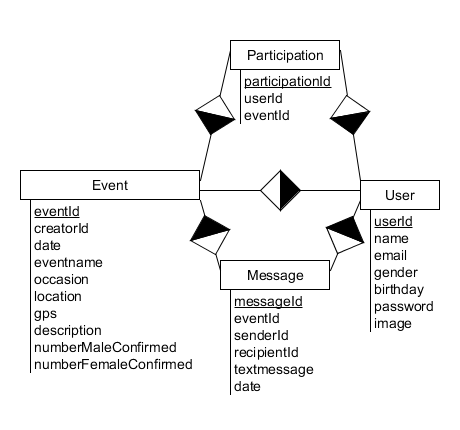
\includegraphics[width=1\textwidth]{Ingo/Bilder/EER-Diagramm.png}
\caption{EER-Diagramm}
\label{fig:EER-Diagramm}
\end{figure}
\section{Der Datengenerator}\label{DerDatengenerator}
�ber den grunds�tzlichen Aufbau des Datengenerators wird im Projekt Datanbankkonfigurationen\footnote{https://dl.dropbox.com/u/608146/ADBC1\%20OLAP.pdf} eingegangen.

Um die Daten schneller in die Tabellen einzuf�gen, werden im Datengenerator die generierten Testdaten anders als in DB-Writer nicht mehr �ber Prepared Statements in die Tabellen eingef�gt, sondern �ber die write-Methode von java.io.Writer in eine Datei geschrieben. Um das umzusetzen, wurde die Komponente DB-Writer durch eine Writer-Komponente ersetzt.

Da sich auch das Data Model in diesem Projekt ge�ndert hat, m�ssen weitere Komponenten des Generators angepasst werden.
Die angepassten Komponenten des Generators zeigt Abbildung \ref{fig:KomponentendiagrammDatengenerator} auf Seite \pageref{fig:KomponentendiagrammDatengenerator}.

\begin{figure}[htp]
\centering
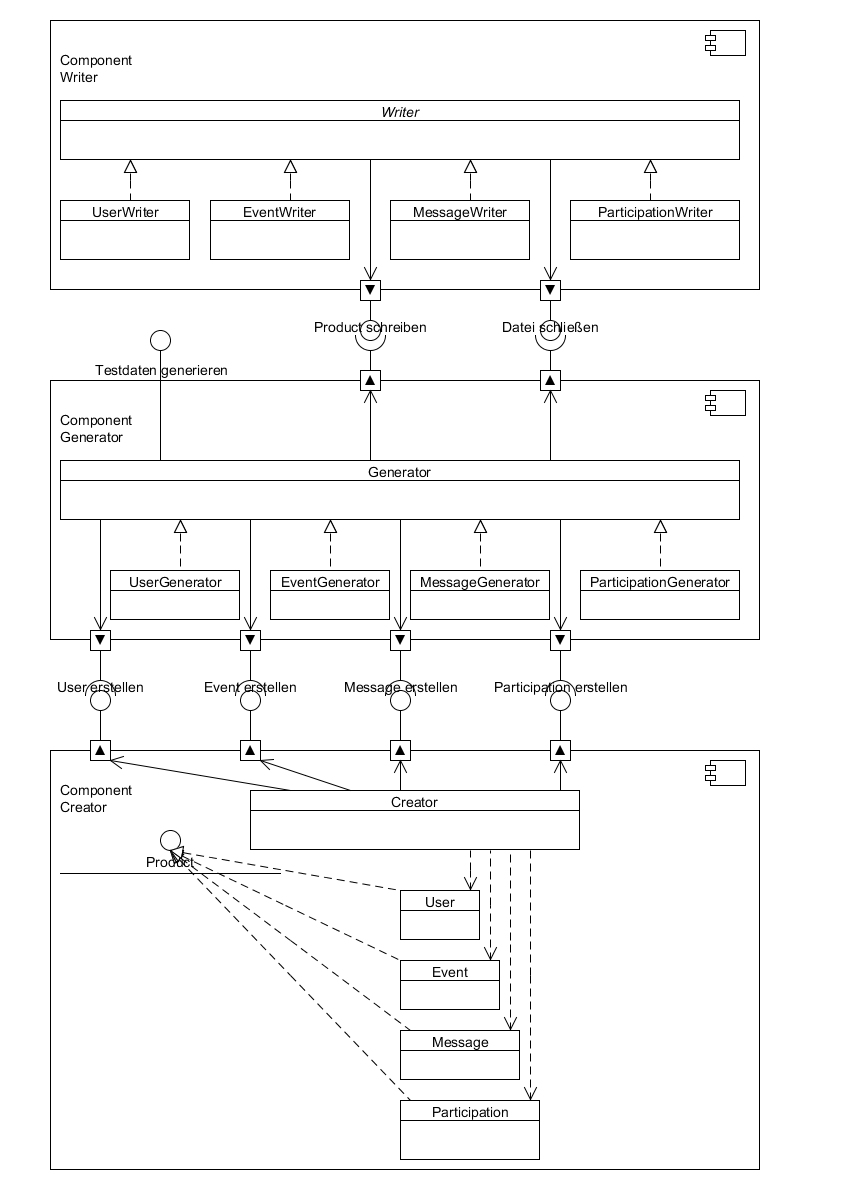
\includegraphics[width=1\textwidth]{Ingo/Bilder/Komponentendiagramm.png}
\caption{Komponentendiagramm Datengenerator}
\label{fig:KomponentendiagrammDatengenerator}
\end{figure}

Die Daten werden im CSV-Format in die jeweilige Datei geschrieben, um sie mit dem Copy-Befehl\footnote{http://www.pgadmin.org/docs/1.4/pg/sql-copy.html} von PostgreSQL in die Tabelle laden zu k�nnen.

\begin{lstlisting}[caption=COPY, firstnumber=1]{code:COPY}
COPY public.User (userId, name, email, gender, birthday, password, image) From 'C:\User.txt' DELIMITER ';'
\end{lstlisting}

Dadurch ergibt sich bei einem Umfang von 3,1 Mio generierter Zeilen im Schnitt eine Zeitersparnis um den Faktor zehn - 66 Sekunden f�r die Generierung und den Import der CSV-Datei in die Tabellen mit COPY, zu 687 Sekunden mit prepared statements.

Das Projekt liegt als Maven-Eclipse-Projekt unter:

https://github.com/rinkdotrink/ComeTogether.git
\section{Datenbankabfragen}\label{Datenbankabfragen}

Query 1: Alle user anzeigen, die am event mit dem eventnamen "`event1"' teilnehmen.

\begin{lstlisting}[caption=Query 1, firstnumber=1]{code:Query1}
Select u.userId, u.name, u.email, u.gender, u.birthday
from public.user u, public.event e, public.participation p
where e.eventname = 'event1'
AND e.eventid = p.eventid
AND p.userid = u.userid;
\end{lstlisting}

Query 2: Alle weiblichen user anzeigen, die zwischen 1986 und 1992 geboren worden und an einem event teilnehmen, dass  zwischen dem 01.01.2013 und dem 01.03.2013 stattfindet, und bei dem numberMaleConfirmed / numberFemaleConfirmed kleiner 0,5 ist.

\begin{lstlisting}[caption=Query 2, firstnumber=1]{code:Query2}
Select u.userId, u.name, u.email, u.gender, u.birthday
from public.user u, public.event e, public.participation p
where u.gender = 'w'
AND u.birthday between '01.01.1986' AND '31.12.1992'
AND e.date between '01.01.2013' AND '01.03.2013'
AND e.eventid = p.eventid
AND p.userid = u.userid
AND e.numberMaleConfirmed / e.numberFemaleConfirmed < 0.5;
\end{lstlisting}

Query 3: Die Anzahl der textmessages gruppiert und absteigend sortiert nach numberFemaleConfirmed, die zwischen dem 01.01.2010 und dem 31.12.2012 geschrieben wurden, in denen das Wort Salsa vorkommt, deren Empf�nger m�nnlich sind und zwischen 1972 und 1982 geboren wurden, deren Absender weiblich sind und die zwischen 1986 und 1992 geboren worden und an einem event teilnehmen, dass  zwischen dem 01.01.2013 und dem 01.03.2013 in einem 100km Radius zu der GPS-Koordinate 11.5833 45.1500 stattfindet und bei dem numberMaleConfirmed / numberFemaleConfirmed kleiner 0,5 ist. Das Ergebnis soll nur die ersten f�nf Treffer liefern.

\begin{lstlisting}[caption=Query 3, firstnumber=1]{code:Query3}
Select e.numberFemaleConfirmed, Count(m.messageid) as anzahlMessages
from public.user u, public.event e, public.participation p, public.message m
where u.gender = 'w'
AND u.birthday between '01.01.1986' AND '31.12.1992'
AND e.date between '01.01.2013' AND '01.03.2013'
AND m.date between '01.01.2010' AND '31.12.2012'
AND m.textmessage like '%Salsa'
AND e.eventid = p.eventid
AND p.userid = u.userid
AND m.senderId = u.userId
AND e.numberMaleConfirmed / e.numberFemaleConfirmed < 0.5
AND DEGREES(acos(cos(RADIANS(90-e.lat))*cos(RADIANS(90-11.5833))+sin(RADIANS(90-e.lat))*
sin(RADIANS(90-11.5833))*cos(RADIANS(e.lon-45.1500))))/360*40074 < 100
AND m.recipientId in
(Select u2.userId
from public.user u2
where u2.gender = 'm'
AND u2.birthday between '01.01.1972' AND '31.12.1982'
)
Group by e.numberFemaleConfirmed
Order by e.numberFemaleConfirmed DESC
Limit 5
\end{lstlisting}
\section{Was ist ein Hints-System?}\label{WasIstEinHintsSystem}
In anderen DBMS wie DB2 oder Oracle kann der Optimizer durch Hinweise (hints) dazu gebracht werden, seinen Ausf�hrungsplan zu ver�ndern.

Der Query in Listing \ref{STRAIGHTJOIN} auf Seite \pageref{STRAIGHTJOIN} gibt in MySQL dem Optimizer den Hinweis, die Tabellen so miteinander zu verkn�pfen, wie sie definiert wurden: Es wird tabA als treibende Tabelle und tabB als innere Tabelle verwendet.

\begin{lstlisting}[caption=STRAIGHT JOIN, firstnumber=1, label=STRAIGHTJOIN]{code:STRAIGHTJOIN}
SELECT STRAIGHT_JOIN *
FROM tabA a, tabB b
WHERE a.id = b.id;
\end{lstlisting}

Wenn MySQL den falschen Index aus einer Menge von m�glichen Indexen nimmt, kann z.B. wie in Listing \ref{USEINDEX} dem Optimizer der Hinweis gegeben werden, nur die im folgenden angegebenden Indexe f�r die Abfrage zu verwenden.

\begin{lstlisting}[caption=USE INDEX, firstnumber=1, label=USEINDEX]{code:USEINDEX}
SELECT * FROM table1 USE INDEX (col1_index,col2_index)
  WHERE col1=1 AND col2=2 AND col3=3;
\end{lstlisting}

Mit dem Hinweis IGNORE INDEX $(col2\_index)$ in Listing \ref{IGNOREINDEX} wird der Optimizer veranlasst, den Index $col3\_index$ f�r die Abfrage nicht zu verwenden.

\begin{lstlisting}[caption=IGNORE INDEX, firstnumber=1, label=IGNOREINDEX]{code:IGNOREINDEX}
SELECT * FROM table1 IGNORE INDEX (col3_index)
  WHERE col1=1 AND col2=2 AND col3=3;
\end{lstlisting}

In PostgreSQL gibt es kein hints-System\footnote{http://wiki.postgresql.org/wiki/OptimizerHintsDiscussion}. Es sind in einem Query keine Konstrukte vorgesehen, dem Planner Hinweise zu geben, wie er den Ausf�hrungsplan erstellen soll.

�berholte Hints - wenn z.B. der Hint f�r die aktuelle Tabellengr��en ungeeignet ist - oder die fehlerhafte Anwendung von Hints - k�nnen zu suboptimalen Ausf�hrungspl�nen f�hren und somit die Ausf�hrungsgeschwindigkeit negativ beeinflussen. Die Fehlerquelle "`menschliches Versagen"' beim Schreiben von Hints wird durch den Verzicht auf ein Hints-System reduziert.

Ohne ein Hints-System wird es allerdings auch schwieriger den Planer verschiedene Ausf�hrungspl�ne erzeugen zu lassen. Und der Planer ist mehr auf sich allein gestellt, der er keine Hilfe von menschlicher Seite in Form von Hints erwarten kann.

Auch wenn der Schreiber des Queries sich auf den Planer verlassen muss, sollte er trotzdem ein paar Dinge beachten, auf die im Folgenden eingegangen wird.
\input{Ingo/Planerverwirrung}
\section{Reihenfolge von Joins erzwingen}\label{ReihenfolgeVonJoinsErzwingen}
Um den Planner zu der angegebenen Join-Reihenfolge zu zwingen, kann das

$join\_collapse\_limit$\footnote{http://www.postgresql.org/docs/current/interactive/explicit-joins.html} auf 1 gesetzt werden.

Um den Planner zu zwingen, Subqueries nicht in einen JOIN umzuandeln, kann das $from\_collapse\_limit$ auf 1 gesetzt werden.

Der Standardwert f�r $join\_collapse\_limit$ und $from\_collapse\_limit$ ist acht. Bei z.B. zw�lf zu verkn�pfenden Tabellen wird keine vollst�ndige Suche mehr nach der besten Joinreihenfolge ausgef�hrt, sondern eine wahrscheinlichkeitstheoretische genetische Suche die nur noch eine begrenzte Zahl von m�glichen Joinreihenfolgen betrachtet. Die genetische Suche braucht weniger Zeit als die vollst�ndige Suche, findet aber nicht zwangsl�ufig die bestm�gliche Joinreihenfolge.
Ab welchem Schwellwert die genetische Suche aktiv wird, kann bei $geqo\_threshold$ gesetzt werden. Der Standardwert ist zw�lf.

Auch wenn $join\_collapse\_limit$ auf den Wert eins gesetzt wird, wird bei folgendem Select die JOIN-Reihenfolge vom Planer bestimmt:

\begin{lstlisting}[caption=Reihenfolge vom Planer bestimmt, firstnumber=1, label=PlanerBestimmt]{code:PlanerBestimmt}
SELECT * FROM a, b, c WHERE a.id = b.id AND b.ref = c.id;
\end{lstlisting}

Erst wenn zwei Tabellen ausdr�cklich mit dem Wort JOIN verkn�pft werden, zwingt das den Planner, diese zwei Tabellen in der gegebenen Reihenfolge zu verkn�pfen:

\begin{lstlisting}[caption=Reihenfolge vom Entwickler bestimmt, firstnumber=1, label=EntwicklerBestimmt]{code:EntwicklerBestimmt}
SELECT * FROM a CROSS JOIN b CROSS JOIN c WHERE a.id = b.id AND b.ref = c.id;
SELECT * FROM a JOIN (b JOIN c ON (b.ref = c.id)) ON (a.id = b.id);
\end{lstlisting}
\section{Ausf�hrungspl�ne f�r Queries mit und ohne Index}\label{AusfuehrungsplaeneFuerQueriesMitUndOhneIndex}

Query 1: Alle user anzeigen, die am event mit dem eventnamen "`event1"' teilnehmen.

\begin{lstlisting}[caption=Query 1, firstnumber=1, label=Query1]{code:Query1}
Select u.userId, u.name, u.email, u.gender, u.birthday
from public.user u, public.event e, public.participation p
where e.eventname = 'event1'
AND e.eventid = p.eventid
AND p.userid = u.userid;
\end{lstlisting}

\begin{lstlisting}[caption=Ausf�hrungsplan Query 1, firstnumber=1, label=aQuery1]{code:aQuery1}
"Hash Join  (cost=254.19..619.78 rows=3595 width=108)"
"  Hash Cond: (p.userid = u.userid)"
"  ->  Hash Join  (cost=231.39..467.41 rows=1498 width=8)"
"        Hash Cond: (p.eventid = e.eventid)"
"        ->  Seq Scan on participation p  (cost=0.00..160.64 rows=9664 width=16)"
"        ->  Hash  (cost=231.00..231.00 rows=31 width=8)"
"              ->  Seq Scan on event e  (cost=0.00..231.00 rows=31 width=8)"
"                    Filter: (eventname = 'event1'::text)"
"  ->  Hash  (cost=16.80..16.80 rows=480 width=108)"
"        ->  Seq Scan on "user" u  (cost=0.00..16.80 rows=480 width=108)"
\end{lstlisting}

mit Prim�r- und Fremdschl�sseln f�r alle Tabellen:

\begin{lstlisting}[caption=Prim�r- und Fremdschl�ssel setzen, firstnumber=1, label=PrimaerUndFremdschluessel]{code:PrimaerUndFremdschluessel}
ALTER TABLE public.event ADD PRIMARY KEY (eventid);
ALTER TABLE public.message ADD PRIMARY KEY (messageid);
ALTER TABLE public.participation ADD PRIMARY KEY (participationid);
ALTER TABLE public.user ADD PRIMARY KEY (userid);
ALTER TABLE event ADD CONSTRAINT event_creatorid FOREIGN KEY (creatorid) REFERENCES public.user (userid) MATCH FULL;
ALTER TABLE message ADD CONSTRAINT message_eventid FOREIGN KEY (eventid) REFERENCES event (eventid) MATCH FULL;
ALTER TABLE message ADD CONSTRAINT message_senderid FOREIGN KEY (senderid) REFERENCES public.user (userid) MATCH FULL;
ALTER TABLE message ADD CONSTRAINT message_recipientid FOREIGN KEY (recipientid) REFERENCES public.user (userid) MATCH FULL;
ALTER TABLE participation ADD CONSTRAINT participation_userid FOREIGN KEY (userid) REFERENCES public.user (userid) MATCH FULL;
ALTER TABLE participation ADD CONSTRAINT participation_eventid FOREIGN KEY (eventid) REFERENCES event (eventid) MATCH FULL;
\end{lstlisting}

\begin{lstlisting}[caption=Ausf�hrungsplan Query 1 mit Prim�r- und Fremdschl�sseln, firstnumber=1, label=aQuery1PrimaerUndFremdschluessel]{code:aQuery1PrimaerUndFremdschluessel}
"Nested Loop  (cost=279.63..495.98 rows=50 width=108)"
"  ->  Hash Join  (cost=279.63..481.63 rows=50 width=8)"
"        Hash Cond: (p.eventid = e.eventid)"
"        ->  Seq Scan on participation p  (cost=0.00..164.00 rows=10000 width=16)"
"        ->  Hash  (cost=279.00..279.00 rows=50 width=8)"
"              ->  Seq Scan on event e  (cost=0.00..279.00 rows=50 width=8)"
"                    Filter: (eventname = 'event1'::text)"
"  ->  Index Scan using user_pkey on "user" u  (cost=0.00..0.27 rows=1 width=108)"
"        Index Cond: (userid = p.userid)"
\end{lstlisting}

sowie Indexen f�r die Fremdschl�ssel:
\begin{lstlisting}[caption=Indexe f�r alle Fremdschl�ssel setzen, firstnumber=1, label=PrimaerUndFremdschluesselUndIndex]{code:PrimaerUndFremdschluesselUndIndex}
CREATE INDEX event_creatorid ON public.event(creatorid);
CREATE INDEX message_eventid ON public.message(eventid);
CREATE INDEX message_senderid ON public.message(senderid);
CREATE INDEX message_recipientid ON public.message(recipientid);
CREATE INDEX participation_userid ON public.participation(userid);
CREATE INDEX participation_eventid ON public.participation(eventid);
\end{lstlisting}

\begin{lstlisting}[caption=Ausf�hrungsplan Query 1 mit Index f�r alle Fremdschl�ssel, firstnumber=1, label=aQuery1PrimaerUndFremdschluesselUndIndexFremdschluessel]{code:aQuery1PrimaerUndFremdschluesselUndIndexFremdschluessel}
"Nested Loop  (cost=0.00..287.57 rows=1 width=38)"
"  ->  Nested Loop  (cost=0.00..287.28 rows=1 width=8)"
"        ->  Seq Scan on event e  (cost=0.00..279.00 rows=1 width=8)"
"              Filter: (eventname = 'event1'::text)"
"        ->  Index Scan using participation_eventid on participation p  (cost=0.00..8.27 rows=1 width=16)"
"              Index Cond: (eventid = e.eventid)"
"  ->  Index Scan using user_pkey on "user" u  (cost=0.00..0.27 rows=1 width=38)"
"        Index Cond: (userid = p.userid)"
\end{lstlisting}

Indexe auf Nicht-Id-Spalten
\begin{lstlisting}[caption=Indexe f�r alle Fremdschl�ssel setzen, firstnumber=1, label=PrimaerUndFremdschluesselUndIndexNichtId]{code:PrimaerUndFremdschluesselUndIndexNichtId}
CREATE INDEX event_date ON public.event(date);
CREATE INDEX event_eventname ON public.event(eventname);
CREATE INDEX event_occasion ON public.event(occasion);
CREATE INDEX event_location ON public.event(location);
CREATE INDEX event_lon ON public.event(lon);
CREATE INDEX event_lat ON public.event(lat);
CREATE INDEX event_numbermaleconfirmed ON public.event(numbermaleconfirmed);
CREATE INDEX event_numberfemaleconfirmed ON public.event(numberfemaleconfirmed);
CREATE INDEX message_textmessage ON public.message(textmessage);
CREATE INDEX message_date ON public.message(date);
CREATE INDEX user_name ON public.user(name);
CREATE INDEX user_email ON public.user(email);
CREATE INDEX user_gender ON public.user(gender);
CREATE INDEX user_birthday ON public.user(birthday);
\end{lstlisting}

\begin{lstlisting}[caption=Ausf�hrungsplan Query 1 mit Indexen f�r alle Fremdschl�ssel, firstnumber=1, label=aQuery1PrimaerUndFremdschluesselUndIndexFremdschluesselNichtId]{code:aQuery1PrimaerUndFremdschluesselUndIndexFremdschluesselNichtId}
"Nested Loop  (cost=0.00..16.84 rows=1 width=38)"
"  ->  Nested Loop  (cost=0.00..16.55 rows=1 width=8)"
"        ->  Index Scan using event_eventname on event e  (cost=0.00..8.27 rows=1 width=8)"
"              Index Cond: (eventname = 'event1'::text)"
"        ->  Index Scan using participation_eventid on participation p  (cost=0.00..8.27 rows=1 width=16)"
"              Index Cond: (eventid = e.eventid)"
"  ->  Index Scan using user_pkey on "user" u  (cost=0.00..0.27 rows=1 width=38)"
"        Index Cond: (userid = p.userid)"
\end{lstlisting}
-------------------------------------------------------------

Query 2: Alle weiblichen user anzeigen, die zwischen 1986 und 1992 geboren worden und an einem event teilnehmen, dass  zwischen dem 01.01.2013 und dem 01.03.2013 stattfindet, und bei dem numberMaleConfirmed / numberFemaleConfirmed kleiner 0,5 ist.

\begin{lstlisting}[caption=Query 2, firstnumber=1, label=Query2]{code:Query2}
Select u.userId, u.name, u.email, u.gender, u.birthday
from public.user u, public.event e, public.participation p
where u.gender = 'w'
AND u.birthday between '01.01.1986' AND '31.12.1992'
AND e.date between '01.01.2013' AND '01.03.2013'
AND e.eventid = p.eventid
AND p.userid = u.userid
AND e.numberMaleConfirmed / e.numberFemaleConfirmed < 0.5;
\end{lstlisting}

\begin{lstlisting}[caption=Ausf�hrungsplan f�r Query 2, firstnumber=1, label=aQuery2]{code:aQuery2}
"Hash Join  (cost=218.37..511.08 rows=2 width=108)"
"  Hash Cond: (e.eventid = p.eventid)"
"  ->  Seq Scan on event e  (cost=0.00..292.60 rows=10 width=8)"
"        Filter: ((date >= '2013-01-01'::date) AND (date <= '2013-03-01'::date) AND (((numbermaleconfirmed / numberfemaleconfirmed))::numeric < 0.5))"
"  ->  Hash  (cost=217.77..217.77 rows=48 width=116)"
"        ->  Hash Join  (cost=20.41..217.77 rows=48 width=116)"
"              Hash Cond: (p.userid = u.userid)"
"              ->  Seq Scan on participation p  (cost=0.00..160.64 rows=9664 width=16)"
"              ->  Hash  (cost=20.40..20.40 rows=1 width=108)"
"                    ->  Seq Scan on "user" u  (cost=0.00..20.40 rows=1 width=108)"
"                          Filter: ((birthday >= '1986-01-01'::date) AND (birthday <= '1992-12-31'::date) AND (gender = 'w'::text))"
\end{lstlisting}


mit Prim�r- und Fremdschl�sseln f�r alle Tabellen:

\begin{lstlisting}[caption=Ausf�hrungsplan Query 2 mit Prim�r- und Fremdschl�sseln, firstnumber=1, label=aQuery2PrimaerUndFremdschluessel]{code:aQuery2PrimaerUndFremdschluessel}
"Nested Loop  (cost=29.96..371.06 rows=10 width=38)"
"  ->  Hash Join  (cost=29.96..235.16 rows=370 width=46)"
"        Hash Cond: (p.userid = u.userid)"
"        ->  Seq Scan on participation p  (cost=0.00..164.00 rows=10000 width=16)"
"        ->  Hash  (cost=29.50..29.50 rows=37 width=38)"
"              ->  Seq Scan on "user" u  (cost=0.00..29.50 rows=37 width=38)"
"                    Filter: ((birthday >= '1986-01-01'::date) AND (birthday <= '1992-12-31'::date) AND (gender = 'w'::text))"
"  ->  Index Scan using event_pkey on event e  (cost=0.00..0.35 rows=1 width=8)"
"        Index Cond: (eventid = p.eventid)"
"        Filter: ((date >= '2013-01-01'::date) AND (date <= '2013-03-01'::date) AND (((numbermaleconfirmed / numberfemaleconfirmed))::numeric < 0.5))"
\end{lstlisting}

sowie Indexen auf Fremdschl�ssel- und Nicht-Id-Spalten:

\begin{lstlisting}[caption=Ausf�hrungsplan Query 2 mit Indexen, firstnumber=1, label=aQuery2PrimaerUndFremdschluesselUndIndexFremdschluesselNichtId]{code:aQuery2PrimaerUndFremdschluesselUndIndexFremdschluesselNichtId}
"Nested Loop  (cost=18.70..359.80 rows=10 width=38)"
"  ->  Hash Join  (cost=18.70..223.90 rows=370 width=46)"
"        Hash Cond: (p.userid = u.userid)"
"        ->  Seq Scan on participation p  (cost=0.00..164.00 rows=10000 width=16)"
"        ->  Hash  (cost=18.24..18.24 rows=37 width=38)"
"              ->  Bitmap Heap Scan on "user" u  (cost=4.98..18.24 rows=37 width=38)"
"                    Recheck Cond: ((birthday >= '1986-01-01'::date) AND (birthday <= '1992-12-31'::date))"
"                    Filter: (gender = 'w'::text)"
"                    ->  Bitmap Index Scan on user_birthday  (cost=0.00..4.97 rows=72 width=0)"
"                          Index Cond: ((birthday >= '1986-01-01'::date) AND (birthday <= '1992-12-31'::date))"
"  ->  Index Scan using event_pkey on event e  (cost=0.00..0.35 rows=1 width=8)"
"        Index Cond: (eventid = p.eventid)"
"        Filter: ((date >= '2013-01-01'::date) AND (date <= '2013-03-01'::date) AND (((numbermaleconfirmed / numberfemaleconfirmed))::numeric < 0.5))"
\end{lstlisting}

-------------------------------------------------------------

Query 3: Die Anzahl der textmessages gruppiert und absteigend sortiert nach numberFemaleConfirmed, die zwischen dem 01.01.2010 und dem 31.12.2012 geschrieben wurden, in denen das Wort Salsa vorkommt, deren Empf�nger m�nnlich sind und zwischen 1972 und 1982 geboren wurden, deren Absender weiblich sind und die zwischen 1986 und 1992 geboren worden und an einem event teilnehmen, dass  zwischen dem 01.01.2013 und dem 01.03.2013 in einem 100km Radius zu der GPS-Koordinate 11.5833 45.15.00 stattfindet und bei dem numberMaleConfirmed / numberFemaleConfirmed kleiner 0,5 ist. Das Ergebnis soll nur die ersten f�nf Treffer liefern.

\begin{lstlisting}[caption=Query 3, firstnumber=1, label=Query3]{code:Query3}
Select e.numberFemaleConfirmed, Count(m.messageid) as anzahlMessages
from public.user u, public.event e, public.participation p, public.message m
where u.gender = 'w'
AND u.birthday between '01.01.1986' AND '31.12.1992'
AND e.date between '01.01.2013' AND '01.03.2013'
AND m.date between '01.01.2010' AND '31.12.2012'
AND m.textmessage like '%Salsa'
AND e.eventid = p.eventid
AND p.userid = u.userid
AND m.senderId = u.userId
AND e.numberMaleConfirmed / e.numberFemaleConfirmed < 0.5
AND DEGREES(acos(cos(RADIANS(90-e.lat))*cos(RADIANS(90-70))+sin(RADIANS(90-e.lat))*
sin(RADIANS(90-70))*cos(RADIANS(e.lon-80))))/360*40074 < 10000
AND m.recipientId in
(Select u2.userId
from public.user u2
where u2.gender = 'm'
AND u2.birthday between '01.01.1972' AND '31.12.1982'
)
Group by e.numberFemaleConfirmed
Order by e.numberFemaleConfirmed DESC
Limit 5
\end{lstlisting}

\begin{lstlisting}[caption=Ausf�hrungsplan f�r Query 3, firstnumber=1, label=aQuery3]{code:aQuery3}
"Limit  (cost=1386.84..1386.86 rows=1 width=12)"
"  ->  GroupAggregate  (cost=1386.84..1386.86 rows=1 width=12)"
"        ->  Sort  (cost=1386.84..1386.84 rows=1 width=12)"
"              Sort Key: e.numberfemaleconfirmed"
"              ->  Nested Loop  (cost=269.91..1386.83 rows=1 width=12)"
"                    Join Filter: (m.senderid = p.userid)"
"                    ->  Hash Join  (cost=239.79..1069.16 rows=3 width=20)"
"                          Hash Cond: (e.eventid = p.eventid)"
"                          ->  Seq Scan on event e  (cost=0.00..829.00 rows=92 width=12)"
"                                Filter: ((date >= '2013-01-01'::date) AND (date <= '2013-03-01'::date) AND (((numbermaleconfirmed / numberfemaleconfirmed))::numeric < 0.5) AND (((degrees(acos(((cos(radians((90::double precision - lat))) * 0.939692620785908::double precision) + ((sin(radians((90::double precision - lat))) * 0.342020143325669::double precision) * cos(radians((lon - 80::double precision))))))) / 360::double precision) * 40074::double precision) < 10000::double precision))"
"                          ->  Hash  (cost=235.16..235.16 rows=370 width=24)"
"                                ->  Hash Join  (cost=29.96..235.16 rows=370 width=24)"
"                                      Hash Cond: (p.userid = u.userid)"
"                                      ->  Seq Scan on participation p  (cost=0.00..164.00 rows=10000 width=16)"
"                                      ->  Hash  (cost=29.50..29.50 rows=37 width=8)"
"                                            ->  Seq Scan on "user" u  (cost=0.00..29.50 rows=37 width=8)"
"                                                  Filter: ((birthday >= '1986-01-01'::date) AND (birthday <= '1992-12-31'::date) AND (gender = 'w'::text))"
"                    ->  Materialize  (cost=30.13..314.39 rows=77 width=16)"
"                          ->  Hash Semi Join  (cost=30.13..314.01 rows=77 width=16)"
"                                Hash Cond: (m.recipientid = u2.userid)"
"                                ->  Seq Scan on message m  (cost=0.00..279.00 rows=1533 width=24)"
"                                      Filter: ((date >= '2010-01-01'::date) AND (date <= '2012-12-31'::date) AND (textmessage ~~ '%Salsa'::text))"
"                                ->  Hash  (cost=29.50..29.50 rows=50 width=8)"
"                                      ->  Seq Scan on "user" u2  (cost=0.00..29.50 rows=50 width=8)"
"                                            Filter: ((birthday >= '1972-01-01'::date) AND (birthday <= '1982-12-31'::date) AND (gender = 'm'::text))"
\end{lstlisting}

\begin{lstlisting}[caption=Ausf�hrungsplan Query 3 mit Prim�r- und Fremdschl�sseln, firstnumber=1, label=aQuery3PrimaerUndFremdschluessel]{code:aQuery3PrimaerUndFremdschluessel}
mit Prim�r- und Fremdschl�sseln f�r alle Tabellen:
"Limit  (cost=546.93..546.95 rows=1 width=12)"
"  ->  GroupAggregate  (cost=546.93..546.95 rows=1 width=12)"
"        ->  Sort  (cost=546.93..546.93 rows=1 width=12)"
"              Sort Key: e.numberfemaleconfirmed"
"              ->  Nested Loop  (cost=333.57..546.92 rows=1 width=12)"
"                    ->  Hash Join  (cost=333.57..535.37 rows=28 width=16)"
"                          Hash Cond: (p.userid = u.userid)"
"                          ->  Seq Scan on participation p  (cost=0.00..164.00 rows=10000 width=16)"
"                          ->  Hash  (cost=333.53..333.53 rows=3 width=24)"
"                                ->  Nested Loop Semi Join  (cost=29.96..333.53 rows=3 width=24)"
"                                      ->  Hash Join  (cost=29.96..315.28 rows=57 width=32)"
"                                            Hash Cond: (m.senderid = u.userid)"
"                                            ->  Seq Scan on message m  (cost=0.00..279.00 rows=1533 width=24)"
"                                                  Filter: ((date >= '2010-01-01'::date) AND (date <= '2012-12-31'::date) AND (textmessage ~~ '%Salsa'::text))"
"                                            ->  Hash  (cost=29.50..29.50 rows=37 width=8)"
"                                                  ->  Seq Scan on "user" u  (cost=0.00..29.50 rows=37 width=8)"
"                                                        Filter: ((birthday >= '1986-01-01'::date) AND (birthday <= '1992-12-31'::date) AND (gender = 'w'::text))"
"                                      ->  Index Scan using user_pkey on "user" u2  (cost=0.00..0.32 rows=1 width=8)"
"                                            Index Cond: (userid = m.recipientid)"
"                                            Filter: ((birthday >= '1972-01-01'::date) AND (birthday <= '1982-12-31'::date) AND (gender = 'm'::text))"
"                    ->  Index Scan using event_pkey on event e  (cost=0.00..0.40 rows=1 width=12)"
"                          Index Cond: (eventid = p.eventid)"
"                          Filter: ((date >= '2013-01-01'::date) AND (date <= '2013-03-01'::date) AND (((numbermaleconfirmed / numberfemaleconfirmed))::numeric < 0.5) AND (((degrees(acos(((cos(radians((90::double precision - lat))) * 0.939692620785908::double precision) + ((sin(radians((90::double precision - lat))) * 0.342020143325669::double precision) * cos(radians((lon - 80::double precision))))))) / 360::double precision) * 40074::double precision) < 10000::double precision))"
\end{lstlisting}


sowie Indexen auf Fremdschl�ssel- und Nicht-Id-Spalten:

\begin{lstlisting}[caption=Ausf�hrungsplan Query 3 mit Indexen, firstnumber=1, label=aQuery3PrimaerUndFremdschluesselUndIndexFremdschluesselNichtId]{code:aQuery3PrimaerUndFremdschluesselUndIndexFremdschluesselNichtId}
"Limit  (cost=355.27..355.29 rows=1 width=12)"
"  ->  GroupAggregate  (cost=355.27..355.29 rows=1 width=12)"
"        ->  Sort  (cost=355.27..355.28 rows=1 width=12)"
"              Sort Key: e.numberfemaleconfirmed"
"              ->  Nested Loop  (cost=18.70..355.26 rows=1 width=12)"
"                    ->  Nested Loop  (cost=18.70..343.72 rows=28 width=16)"
"                          ->  Nested Loop Semi Join  (cost=18.70..322.27 rows=3 width=24)"
"                                ->  Hash Join  (cost=18.70..304.02 rows=57 width=32)"
"                                      Hash Cond: (m.senderid = u.userid)"
"                                      ->  Seq Scan on message m  (cost=0.00..279.00 rows=1533 width=24)"
"                                            Filter: ((date >= '2010-01-01'::date) AND (date <= '2012-12-31'::date) AND (textmessage ~~ '%Salsa'::text))"
"                                      ->  Hash  (cost=18.24..18.24 rows=37 width=8)"
"                                            ->  Bitmap Heap Scan on "user" u  (cost=4.98..18.24 rows=37 width=8)"
"                                                  Recheck Cond: ((birthday >= '1986-01-01'::date) AND (birthday <= '1992-12-31'::date))"
"                                                  Filter: (gender = 'w'::text)"
"                                                  ->  Bitmap Index Scan on user_birthday  (cost=0.00..4.97 rows=72 width=0)"
"                                                        Index Cond: ((birthday >= '1986-01-01'::date) AND (birthday <= '1992-12-31'::date))"
"                                ->  Index Scan using user_pkey on "user" u2  (cost=0.00..0.32 rows=1 width=8)"
"                                      Index Cond: (userid = m.recipientid)"
"                                      Filter: ((birthday >= '1972-01-01'::date) AND (birthday <= '1982-12-31'::date) AND (gender = 'm'::text))"
"                          ->  Index Scan using participation_userid on participation p  (cost=0.00..7.02 rows=10 width=16)"
"                                Index Cond: (userid = u.userid)"
"                    ->  Index Scan using event_pkey on event e  (cost=0.00..0.40 rows=1 width=12)"
"                          Index Cond: (eventid = p.eventid)"
"                          Filter: ((date >= '2013-01-01'::date) AND (date <= '2013-03-01'::date) AND (((numbermaleconfirmed / numberfemaleconfirmed))::numeric < 0.5) AND (((degrees(acos(((cos(radians((90::double precision - lat))) * 0.939692620785908::double precision) + ((sin(radians((90::double precision - lat))) * 0.342020143325669::double precision) * cos(radians((lon - 80::double precision))))))) / 360::double precision) * 40074::double precision) < 10000::double precision))"
\end{lstlisting}
\section{Was tun bei langsamen Ausf�hrungspl�nen?}\label{WasTunBeiLangsamenAusfuehrungsplaenen}

\begin{itemize}
\item Um dem Planer keine falschen Hinweise zu geben, sollten keine Hints verwendet werden.

\item Autoanalyze aktivieren\\
Der Planner kann nur dann optimierte Ausf�hrungspl�ne erzeugen, wenn er gen�gend Statistiken �ber die gef�llten Tabellen besitzt. Deswegen m�ssen regelm��ig Statistiken erstellt werden. In PostgreSQL geht das mit analyze. Analyze sammelt Informationen �ber den F�llstand der Tabellen, die h�ufigsten Werte in jeder Spalten und die wahrscheinliche Verteilung der Werte in einer Spalte.
Mit diesen Statistiken kann der Planer dann den passenden JOIN-Algorithmus und die passende JOIN-Order w�hlen.
Um nach bestimmten Abst�nden automatisch analyze aufzurufen, gibt es autoanalyze.

\item Autovacuum aktivieren \\
Mit autovacuum = on in der postgresql.conf kann autovacuum aktiviert werden.

\item Indexe verwenden \\
Es kann z.B. der Entwickler geeignete Indexe anlegen, sodass das DBMS diese verwenden kann, um performantere Ausf�hrungspl�ne zu erzeugen.

\item Mehrspaltige Indexe verwenden, wenn dadurch ein performanterer Ausf�hrungs\-plan erzeugt werden kann.

\item Keine zu intensiven Rechnungen in SQL formulieren.

\item Partitioning verwenden.

\item Die Struktur der Tabellen �berdenken, wenn mehr als 8 Tabellen miteinander verkn�pft werden.

\item Herausfinden, warum der Planner einen langsamen Plan erzeugt, anstatt durch Planner-Hints der Frage aus dem Weg zu gehen.

\item Es kann sein, dass jemand ung�nstige Werte f�r die Parameter in der postgresql.conf gesetzt hat.

\item Bei einem zu kleinen Wert f�r $join\_collapse\_limit$ in der postgresql.conf, verbunden mit der expliziten Verkn�pfung von Tabellen mit dem Wort Join, ist der Planner gezwungen, eine vorgegebene aber u.U. ung�nstige Join-Reihenfolge zu verwenden.

\item Um dem Planner nicht ausversehen zu etwas zu zwingen, sollten bei einem Innerjoin die Tabellen nicht explizit mit dem Wort JOIN verkn�pfen werden, sondern es sollten die Tabellen einfach getrennt durch ein Komma angeben werden:

\begin{lstlisting}[caption=Inner-Join, firstnumber=1, label=gtlt]{code:gtlt}
SELECT * FROM a, b, c WHERE a.id = b.id AND b.ref = c.id;
\end{lstlisting}

\item Bei einem zu kleinen Wert f�r $from\_collapse\_limit$ in der postgresql.conf, verbunden mit vielen Subqueries, kann der Planner die Subqueries nicht aufl�sen. Dabei sollte der Planner Subqueries zu Joins aufl�sen, da sonst erst das komplette Ergebnis des Subquerys erstellt werden muss, bevor mit der Tabelle weitergearbeitet werden kann.
\end{itemize}
\section{Zusammenfassung}\label{Zusammenfassung}
Der Planer von PostgreSQL ist so ausgereift, dass dessen Entwickler bewusst auf ein Hints-System verzichten. Es wird davon ausgegangen, dass der Planer umso bessere Ausf�hrungspl�ne macht, je mehr Entscheidungsfreiheit er bei der Planerstellung hat. Diese Entscheidungsfreiheit w�rden durch Hints eingeschr�nkt. Ausf�hrungsplanoptimierung beschr�nkt sich bei PostgreSQL vor allem darauf, sicherzustellen, dass der Planer immer aktuelle Statistiken hat und ihm m�glichst viele Indexe zur Verf�gung stehen, aus denen er die seiner meiner nach Besten w�hlen kann, um einen effizienten Ausf�hrungsplan zu erstellen.
\section{Ausblick}\label{Ausblick}
In einem weiteren Projekt k�nnte man die Ausf�hrungspl�ne bei Tabellen mit Partitioning untersuchen.

Es k�nnte auch die Arbeitsweise des Planers untersucht werden, wenn mehr als f�nfzehn Tabellen miteinander verkn�pft werden und er mit einer genetischen Suche nach einem effizienten Auf�hrungsplan sucht.

Es k�nnte gezeigt werden, welchen Einfluss der F�llstand einer Tabelle und die Verteilung der Werte in einer einzelnen Spalte auf die Generierung eines Ausf�hrungsplanes hat.



%\chapter{Theoretische Grundlagen}
%Die f\"{u}r den Untersuchungsgegenstand relevanten Themen, die \"{u}ber die
%grundlegenden Studieninhalte hinausgehen; oft auch anwendungsspezifische Aspekte - %ca. 6 Seiten

%\chapter{Ist-Analyse}
%Welche Defizite sollen mit der Arbeit behoben werden, welche nicht? %Pr\"{a}zisierung
%der Zielstellung - ca. 6 Seiten

%\chapter{L\"{o}sungskonzept}
%Wie sollen die Defizite behoben werden? Methoden, fachliche Auseinandersetzung
%mit alternativen Ans\"{a}tzen und Auffassungen, Systembeschreibung (Architektur,
%Vorgehensmodell, \ldots) - ca. 12 Seiten

%\chapter{Implementierung}
%Umsetzung des L\"{o}sungskonzepts, Begr\"{u}ndung der verwendeten Technologien - %ca. 8
%Seiten

%\chapter{Ergebnisse}
%Objektive Bewertung der vorliegenden L\"{o}sung, diverse Testverfahren,
%Nutzerbefragungen - ca. 4 Seiten

%\chapter{Fazit und Ausblick}
%Zusammenfassung s\"{a}mtlicher Ergebnisse in Bezug auf die Zielerf\"{u}llung und
%Vorschl\"{a}ge f\"{u}r weiterf\"{u}hrende Arbeiten - ca. 2 Seiten

\bibliographystyle{alphadin}
\begin{appendix}
\newpage
\pagestyle{appendixAStyle}
\chapter{Codebeispiele}
\begin{lstlisting}[caption=alle Tabellen erstellen, firstnumber=1]{code:TabellenErstellen}
CREATE TABLE "user"
(
  userid bigint,
  name text,
  email text,
  gender text,
  birthday date,
  password text,
  image text
)
WITH (
  OIDS=FALSE
);
ALTER TABLE "user"
  OWNER TO postgres;

CREATE TABLE event
(
  eventid bigint NOT NULL,
  creatorid bigint,
  date date,
  eventname text,
  occasion text,
  location text,
  lon double precision,
  lat double precision,
  description text,
  numbermaleconfirmed int,
  numberfemaleconfirmed int
)
WITH (
  OIDS=FALSE
);
ALTER TABLE event
  OWNER TO postgres;

CREATE TABLE message
(
  messageid bigint,
  eventid bigint,
  senderid bigint,
  recipientid bigint,
  textmessage text,
  date date
)
WITH (
  OIDS=FALSE
);
ALTER TABLE message
  OWNER TO postgres;

CREATE TABLE participation
(
  participationid bigint,
  userid bigint,
  eventid bigint
)
WITH (
  OIDS=FALSE
);
ALTER TABLE participation
  OWNER TO postgres;
\end{lstlisting}

\begin{lstlisting}[caption=Datenimport �ber COPY, firstnumber=1]{code:COPY}
COPY public.Event (eventid, creatorid, date, eventname, occasion, location, lon, lat, description, numbermaleconfirmed, numberfemaleconfirmed) From 'C:\Event.txt' DELIMITER ';';
COPY public.Message (messageid, eventid, senderid, recipientid, textmessage, date) From 'C:\Message.txt' DELIMITER ';';
COPY public.Participation (participationid, userid, eventid) From 'C:\Participation.txt' DELIMITER ';';
COPY public.User (userId, name, email, gender, birthday, password, image) From 'C:\User.txt' DELIMITER ';';
\end{lstlisting}


\begin{lstlisting}[caption=Prim�r- und Fremdschl�ssel hinzuf�gen, firstnumber=1]{code:PrimaryForeignKeys}
ALTER TABLE public.event ADD PRIMARY KEY (eventid);
ALTER TABLE public.message ADD PRIMARY KEY (messageid);
ALTER TABLE public.participation ADD PRIMARY KEY (participationid);
ALTER TABLE public.user ADD PRIMARY KEY (userid);

ALTER TABLE event ADD CONSTRAINT event_creatorid FOREIGN KEY (creatorid) REFERENCES public.user (userid) MATCH FULL;
ALTER TABLE message ADD CONSTRAINT message_eventid FOREIGN KEY (eventid) REFERENCES event (eventid) MATCH FULL;
ALTER TABLE message ADD CONSTRAINT message_senderid FOREIGN KEY (senderid) REFERENCES public.user (userid) MATCH FULL;
ALTER TABLE message ADD CONSTRAINT message_recipientid FOREIGN KEY (recipientid) REFERENCES public.user (userid) MATCH FULL;
ALTER TABLE participation ADD CONSTRAINT participation_userid FOREIGN KEY (userid) REFERENCES public.user (userid) MATCH FULL;
ALTER TABLE participation ADD CONSTRAINT participation_eventid FOREIGN KEY (eventid) REFERENCES event (eventid) MATCH FULL;
\end{lstlisting}


\begin{lstlisting}[caption=Indexe auf Spalten legen, firstnumber=1]{code:Indexe}
CREATE INDEX event_creatorid ON public.event(creatorid);
CREATE INDEX message_eventid ON public.message(eventid);
CREATE INDEX message_senderid ON public.message(senderid);
CREATE INDEX message_recipientid ON public.message(recipientid);
CREATE INDEX participation_userid ON public.participation(userid);
CREATE INDEX participation_eventid ON public.participation(eventid);

CREATE INDEX event_date ON public.event(date);
CREATE INDEX event_eventname ON public.event(eventname);
CREATE INDEX event_occasion ON public.event(occasion);
CREATE INDEX event_location ON public.event(location);
CREATE INDEX event_lon ON public.event(lon);
CREATE INDEX event_lat ON public.event(lat);
CREATE INDEX event_numbermaleconfirmed ON public.event(numbermaleconfirmed);
CREATE INDEX event_numberfemaleconfirmed ON public.event(numberfemaleconfirmed);

CREATE INDEX message_textmessage ON public.message(textmessage);
CREATE INDEX message_date ON public.message(date);

CREATE INDEX user_name ON public.user(name);
CREATE INDEX user_email ON public.user(email);
CREATE INDEX user_gender ON public.user(gender);
CREATE INDEX user_birthday ON public.user(birthday);
\end{lstlisting}
\end{appendix}

\newpage
\chapter{Work Packages}


\begin{table}[h] \begin{flushleft}  \begin{tabular}{|l||c|c|c|c|c|c|}
\hline
\textbf{Work Packages}		&	\textbf{C. Ochmann}	& \textbf{I. K�rner}  \\ \hline \hline
abstract   	      &                     & x       \\
introduction&                                      & x  \\ 
requirements engineering& x & x  \\ 
previous work& & x  \\ 
design&                                      & x  \\ 
miscellaneous& & x  \\ 
programming environment& & x  \\ 
backend  &                             		      & x \\
frontend &  x & \\
maven-android-projekt &  x & \\
database&                              & x \\ 
conclusion&                           x       & x  \\
\hline \hline
\end{tabular} \end{flushleft} \caption{Work Packages} \end{table}



\newpage
\chapter{Eigenst�ndigkeitserkl�rung}
Hiermit erkl�re ich, dass ich diese Arbeit selbst�ndig verfasst habe. Mir ist bekannt, dass jede Form des Plagiats mit der Note 5 (Betrugsversuch) bewertet wird.

\begin{tabular}{@{}p{6.0cm}p{6.0cm}}	  		  		 	
	  		 & \\
	  		 & \\
				  			\textbf{Ochmann, Christof} &               Unterschrift:\\				 
				 &\\
				 & \\
				  			\textbf{K�rner, Ingo}   	&                     Unterschrift:\\			
\end{tabular}
\end{document}
